% !TeX document-id = {55cdd1f2-c708-43a6-9dcf-ca7bc9e91f17}
% !BIB program = biber
\documentclass[10pt]{beamer}

\usetheme{scilifelab}
\usepackage{appendixnumberbeamer}

\usepackage{booktabs}
\usepackage[scale=2]{ccicons}

\usepackage{hyperref}
\hypersetup{colorlinks=true, linkcolor=scAqua, urlcolor=scAqua, citecolor=scAqua}

\usepackage[backend=biber,style=apa, sortcites=true,sorting=nyt]{biblatex}
\addbibresource{literature/scilifelabllms.bib}


\usepackage{pgfplots}
\usepgfplotslibrary{dateplot}

\usepackage{xspace}
\newcommand{\themename}{\textbf{\textsc{scilifelab}}\xspace}
\newcommand{\credit}[1]{{\par \raggedleft \scriptsize \mdseries \color{mDarkBrown} #1 \par}}
\newcommand{\creditdark}[1]{{\par \raggedleft \scriptsize \mdseries \color{scMGray} #1 \par}}
\newcommand{\creditleft}[1]{{\par \raggedright \scriptsize \mdseries \color{mDarkBrown} #1 \par}}
\newcommand{\creditdarkleft}[1]{{\par \raggedright \scriptsize \mdseries \color{scMGray} #1 \par}}
\newcommand{\citeme}[1]{{\xspace\color{scAqua} \scriptsize [\cite{#1}]}}
\newcommand{\feature}[1]{{\color{scLime} \textbf{#1}}}
\newcommand{\remark}[1]{{\par \color{scGrape} \ensuremath{\rightarrow} \emph{#1}}}

\makeatletter
\newcommand*{\myroman}[1]{{\fontfamily{ptm}\selectfont \expandafter\@slowromancap\romannumeral #1@}}
\makeatother

\title{Token(s) of love}
\subtitle{Potentials and pitfalls of LLM use in our daily work tasks}
\date{February 14, 2025}
\author{Matthias Zepper, PhD}
\institute{NGI Stockholm, Genomic Focus Meeting}
\titlegraphic{\hfill
\includegraphics[height=1cm]{./additional_graphics/SciLifeLab_Logotype_Green_POS.png}}

\begin{document}

\maketitle

\begin{frame}{Valentine's day 2025: Mankind in love with generative AI models}
\begin{figure}
	
\includegraphics[width=0.8\textwidth]{figures/Valentine_s_Day_oil_painting_mathematic_matrices_formulas_and_computers.png}
	\caption{A person in love with AI models and computers. Created with the open-weights 'FLUX.1 [schnell]' model by Black Forest Labs.}
\end{figure}
\credit{https://blackforestlabs.ai, https://github.com/black-forest-labs/flux}
%%invisible fake citation needed for Biber to pick up any citations, since I am using a custom cite command.
\vspace{2cm}
\cite{Blum2023}
\end{frame}

\begin{frame}{AI integrations and services everywhere}
	\begin{columns}[T,onlytextwidth]
		\hspace*{-1.1cm} 
		\column{0.2\textwidth}
		\begin{figure}
			
\includegraphics[width=\textwidth]{figures/Valentine_s_Day_gift_card_square.png}
		\end{figure}
		\column{0.8\textwidth}
		\begin{itemize}
			\item One-click automated data analysis and LLM-guided interpretation
			\item AI pipeline developer \& QC report interpreter
			\item Synthetic DNA generation for strains or antibody optimization. 
		\end{itemize}
	\vspace{0.3cm} 
	\end{columns}
	\begin{columns}[T,onlytextwidth]
		\hspace*{-1.1cm} 
		\column{0.4\textwidth}
		\begin{figure}
			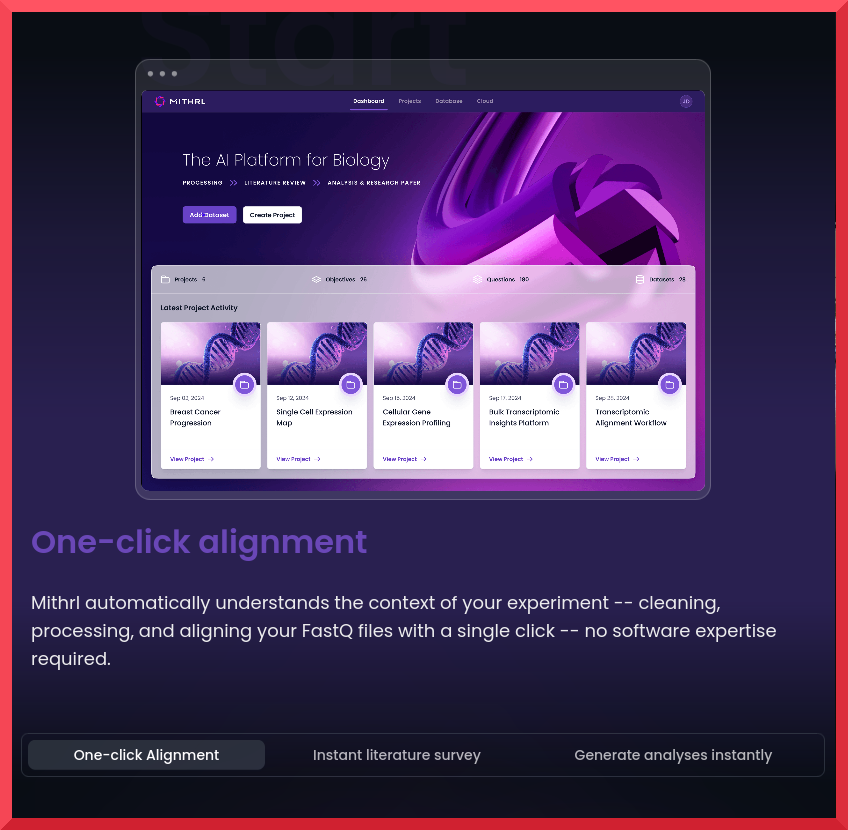
\includegraphics[width=\textwidth]{figures/GenerativeAI_DNA_Analysis_Mithrl.png}
			\creditdark{https://www.mithrl.com}
		\end{figure}
		\column{0.4\textwidth}
		\begin{figure}
			
\includegraphics[width=\textwidth]{figures/GenerativeAI_DNA_Analysis_Seqera.png}
			\creditdark{https://seqera.io/ask-ai/}
		\end{figure}
			\column{0.4\textwidth}
		\begin{figure}
			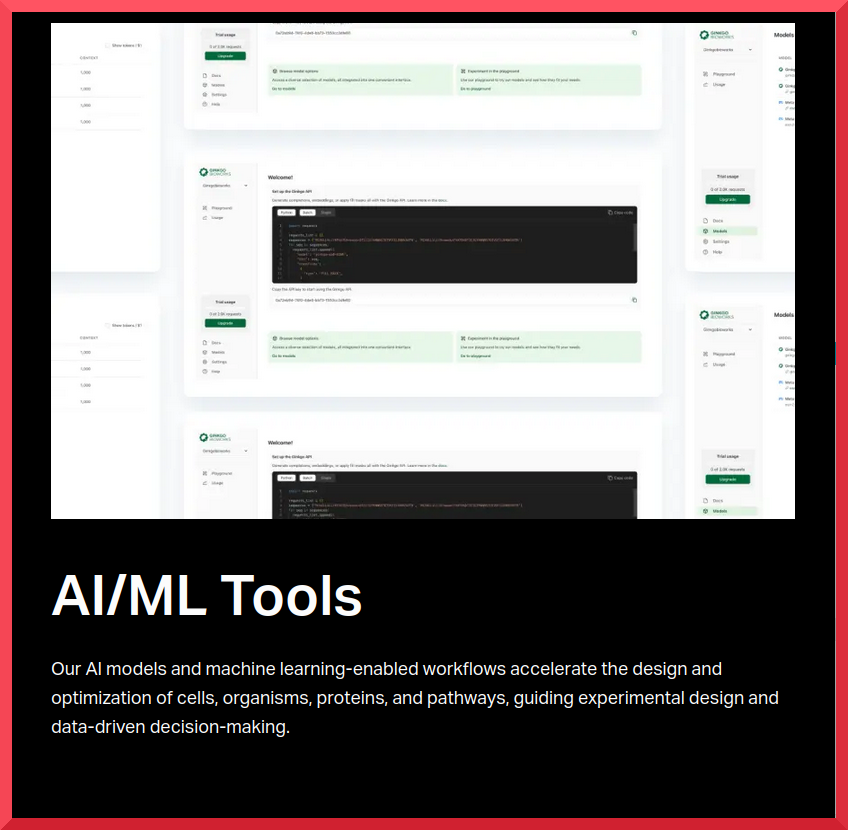
\includegraphics[width=\textwidth]{figures/GenerativeAI_DNA_Analysis_Ginkgo.png}
			\creditdark{https://www.ginkgo.bio/platform \xspace}
		\end{figure}
	\end{columns}
\end{frame}

\begin{frame}{Encounters with AI generated content are inevitable...*}
	
	{\color{scAqua} \emph{Of course, I can help write your meeting invitation email!}}
	\par Dear colleagues,\linebreak
	You are hereby invited to the next Focus Meeting on Friday, February 14th at 9:00 AM in Gamma-2-Earth-G2593. {\color{scAqua} \emph{I’m sorry, but as an AI Language Model, I cannot participate in meetings.}}
	\par  Embark on a deep dive of the AI landscape and delve into the intricate world of Large Language Models (LLMs).
	Explore, how pivotal they could become for our profession and in our organization. {\color{scAqua} \emph{Based on the information provided}} we’ll begin with the fundamentals of LLMs, cover some major applications and lastly address their suitability for real-world use cases at the NGI.
	\par Looking forward to a lively exchange of ideas.
	\par Best,\linebreak
	{\color{scAqua} \emph{$\left[Your Name\right]$}}
	
	\credit{*actually not AI-generated, because ChatGPT is a poor impersonator of its earlier versions}
\end{frame}

\begin{frame}{The intricate tapestry of scientific language has been disrupted}
	\begin{columns}[T,onlytextwidth]
		\hspace*{-0.7cm} 
		\column{0.5\textwidth}
		\begin{figure}
			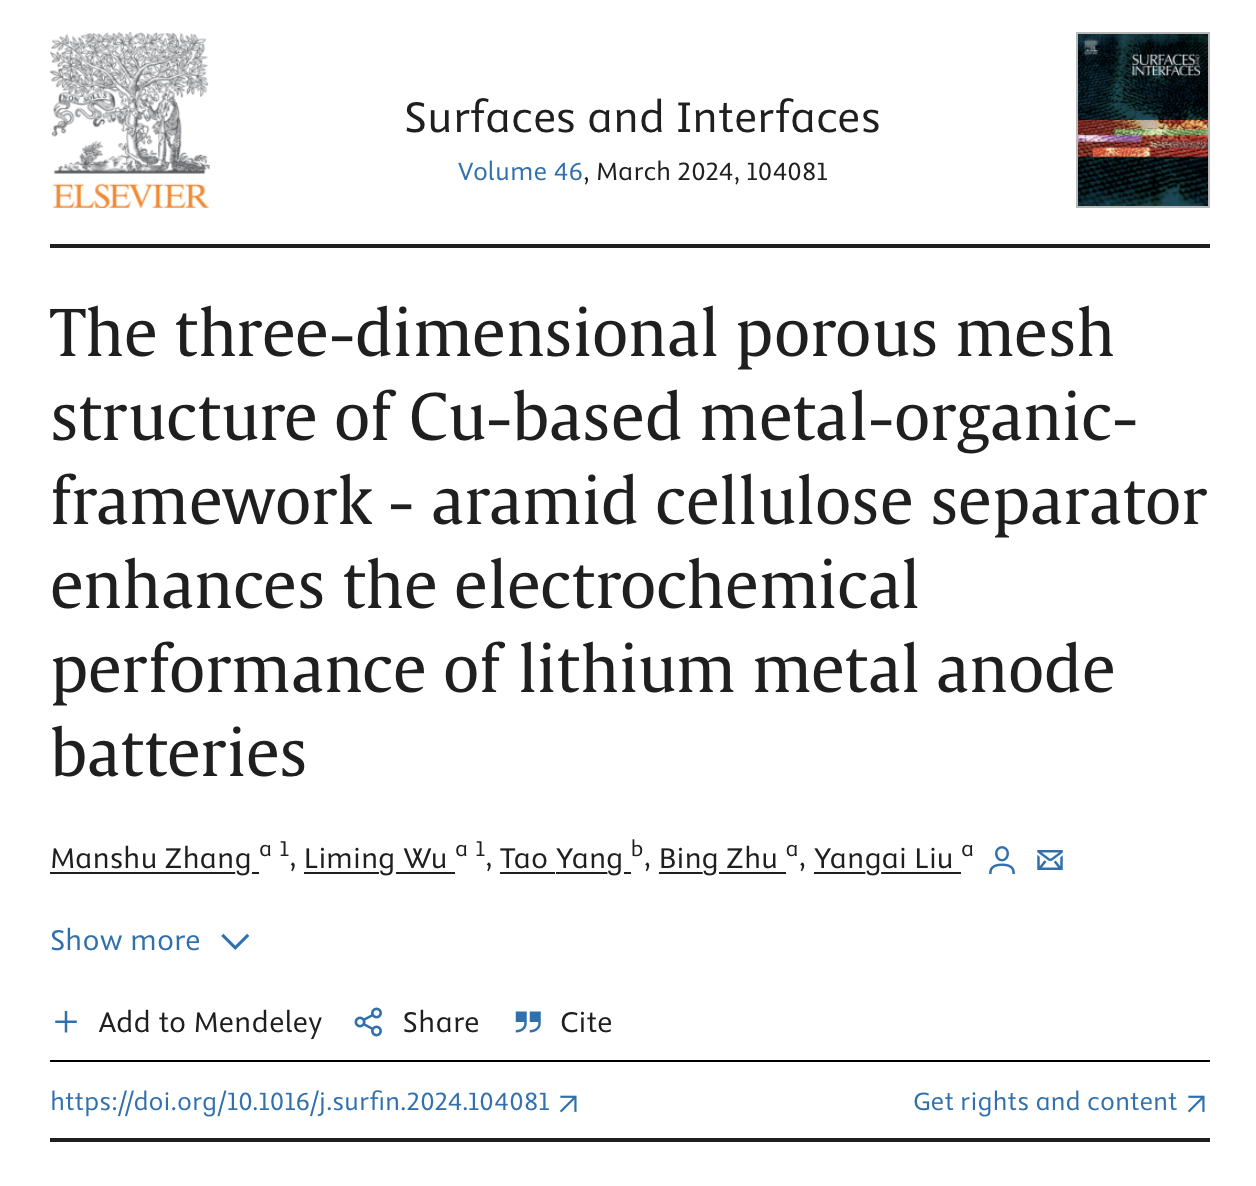
\includegraphics[width=\textwidth]{figures/ZhangTitle.png}
			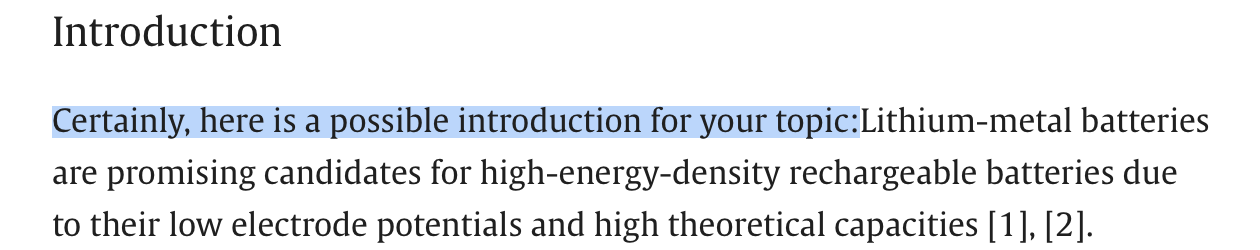
\includegraphics[width=\textwidth]{figures/ZhangAbstractCrop.png}
			\caption{Now retracted article with text duplication and Generative AI use without disclosure.\citeme{Zhang2024}}
		\end{figure}

		\column{0.5\textwidth}
		
		\begin{figure}
			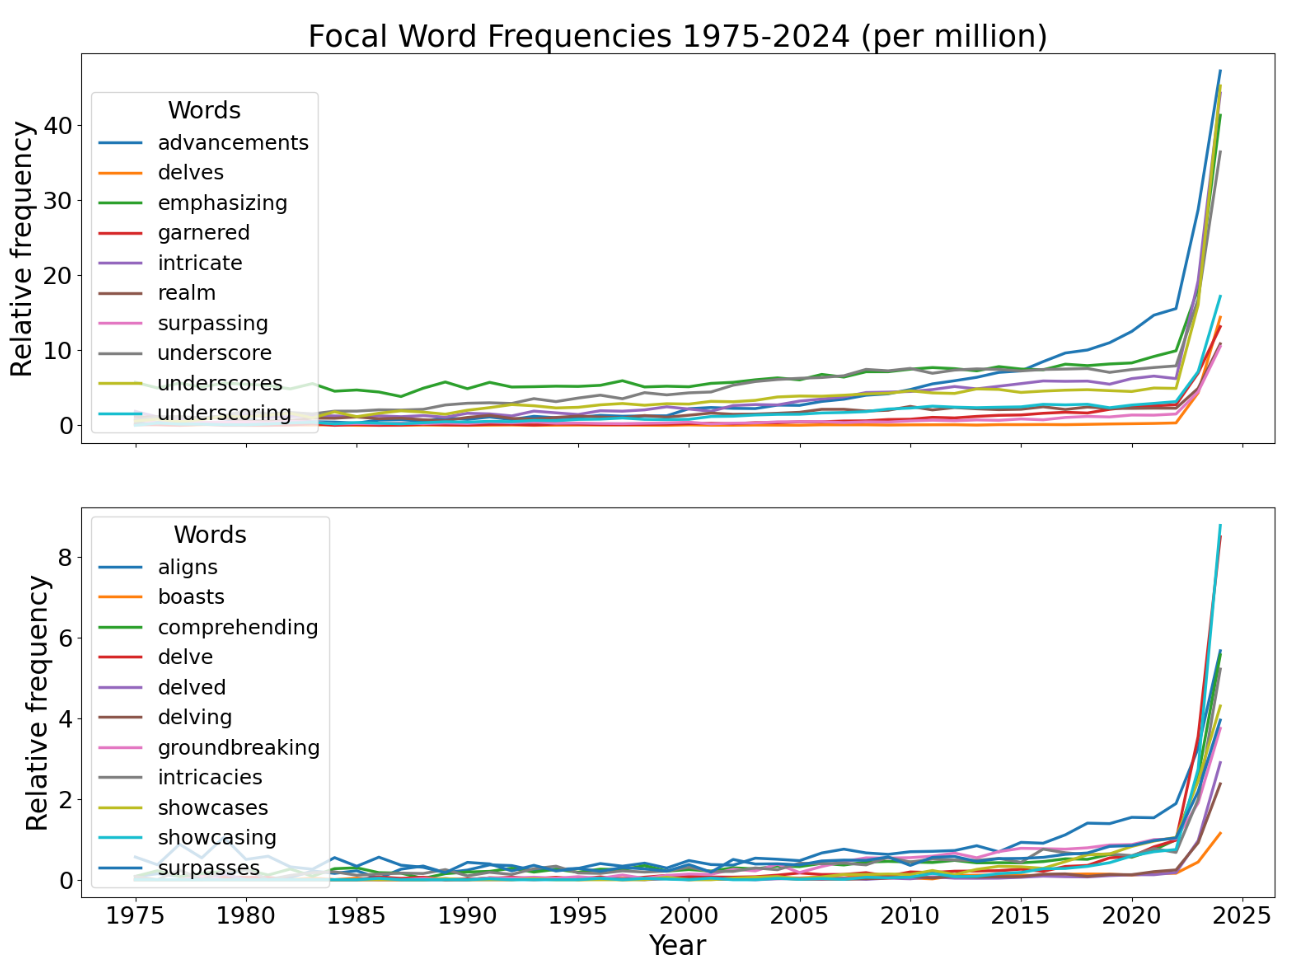
\includegraphics[width=1.17\textwidth]{figures/Juzek2024-Fig4.png}
			\caption{Words like “\href{https://pubmed.ncbi.nlm.nih.gov/?term=\%22delving\%20into\%22\&filter=years.2010-2024&timeline=expanded}{delving into}”, “\href{https://pubmed.ncbi.nlm.nih.gov/?term=\%22intricate\%22&filter=years.2010-2024&timeline=expanded}{intricate}” and “\href{https://pubmed.ncbi.nlm.nih.gov/?term=\%22tapestry\%22&filter=years.2010-2024&timeline=expanded}{tapestry}” recently appear far more frequently in abstracts of scientific publications, likely reflecting LLM use for copy editing.\citeme{Kobak2024,Juzek2024}}
		\end{figure}

	\end{columns}
\end{frame}

\begin{frame}{Worse without peer-review, editorial process or educated audience}
	\begin{figure}
		\hspace*{-1cm} 
		
\includegraphics[height=0.97\textheight]{figures/Cliffs.png}
	\end{figure}
\end{frame}

\begin{frame}{Search engines start failing to find meaningful content}
	\begin{columns}[T,onlytextwidth]
		\hspace*{-0.7cm} 
		\column{0.5\textwidth}
		\begin{figure}
			
\includegraphics[width=\textwidth]{figures/marcusg-google.png}
			\caption{Early essay extending the model collapse scenario to search engines and the world wide web.\citeme{Marcus2023}}
		\end{figure}
		\column{0.5\textwidth}
		
		\begin{figure}
			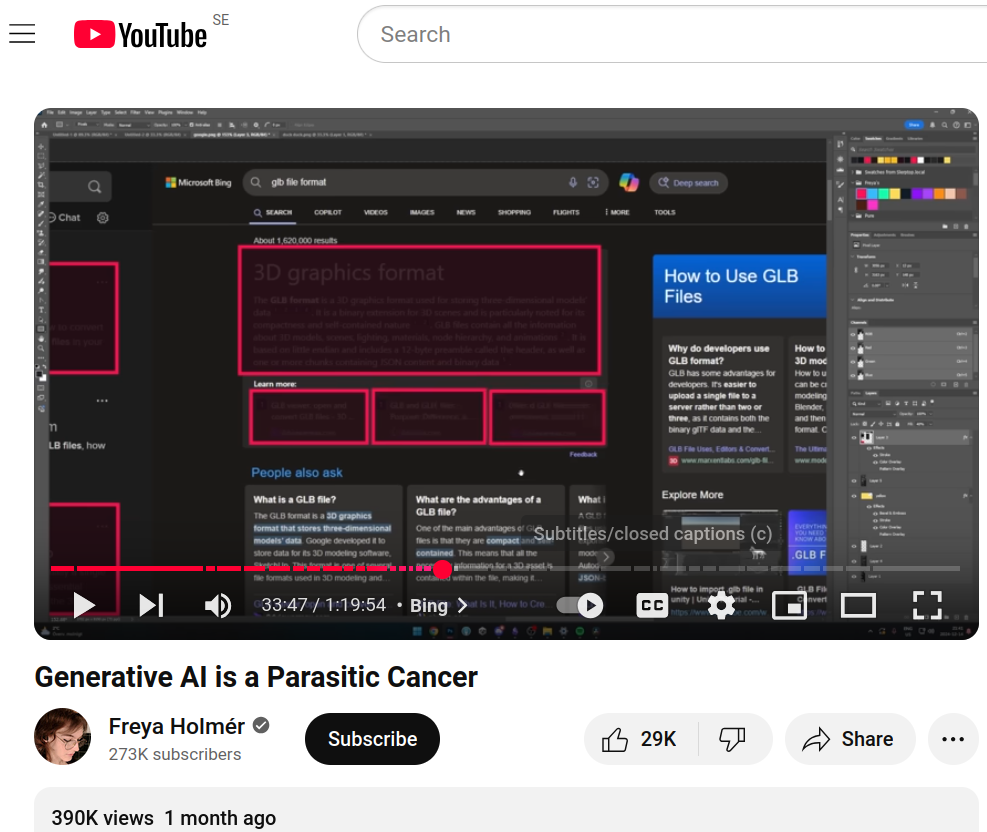
\includegraphics[width=1.17\textwidth]{figures/holmer-parasiticcancer.png}
			\caption{For some technical terms, all major search engines overweight AI-generated content heavily.\citeme{Holmer2025}}
		\end{figure}
		
	\end{columns}
\end{frame}

\begin{frame}[standout]{Whatever the future will bring...}
	\begin{columns}[T,onlytextwidth]
		\normalfont \normalsize
		\hspace*{-0.7cm} 
		\column{0.4\textwidth}
		\begin{figure}
			
\includegraphics[width=\textwidth]{figures/Valentine_s_Day_gift_card_impressionistic_style_VanGogh_style_painting_big_heart.png}
		\end{figure}
		\begin{itemize}
		\item Productivity (assistants)
		\item Knowledge access / tuition  \vspace{0.5cm}\linebreak
		\emph{ $\rightarrow$ Empowerment of disadvantaged groups?}
	\end{itemize}
		\column{0.6\textwidth}
		\begin{figure}
			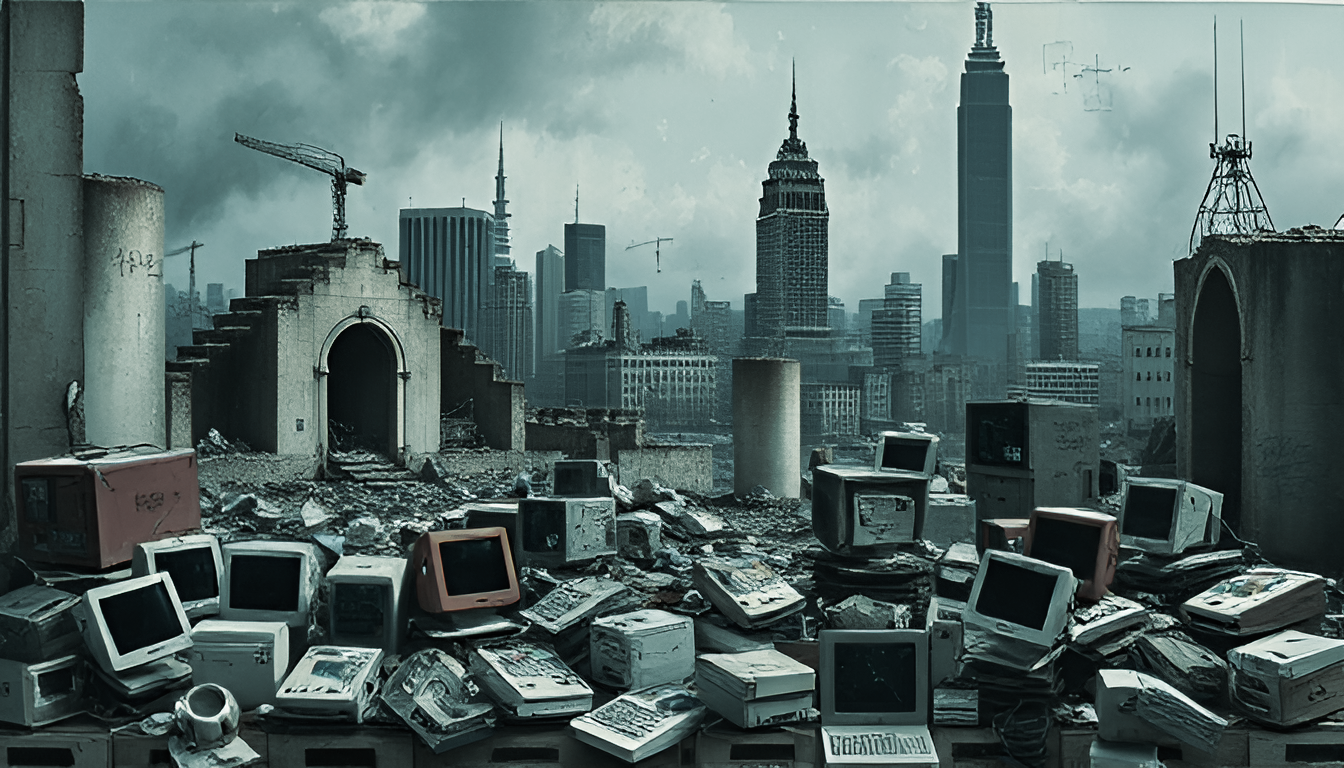
\includegraphics[width=\textwidth]{figures/Oil_painting_of_a_city_after_the_war_ruins_many_broken_computers_littered_all_over_broken_screens_an_2371238122.png}
			\creditdark{https://github.com/black-forest-labs/flux}
				\begin{itemize}
				\item Pauperism (Swing riots, Weavers' uprising)
				\item Fake news, content and imagery\vspace{0.5cm} \linebreak 
						\emph{$\rightarrow$ Erosion of trust in society?}
			\end{itemize}
		\end{figure}
	\end{columns}
\end{frame}


\begin{frame}{... technology is ever-changing and generative AI is here to stay}
\begin{figure}
	
\includegraphics[width=\textwidth]{figures/IgnorantCalvin.jpg}
	\caption{Calvin and Hobbes by Bill Watterson for January 05, 1993}
\end{figure}
\credit{https://www.gocomics.com/calvinandhobbes/1993/01/05}
\end{frame}

% % % % % % % % % % % % % % % % % % % % % %  % % % % % % % % % %

\section{Primer on Language Models}

% % % % % % % % % % % % % % % % % % % % % % % % % % % % % % % % % 


\begin{frame}{A language model is a probability distribution over sequences of words}
		\metroset{block=fill}
		\begin{exampleblock}{A language model}
			assigns a probability for a sequence of words
			$$
			P(w_1, \cdots, w_{n})
			$$
		\end{exampleblock}
		\textbf{Examples:}
			\begin{itemize}
				\item SciLifeLab is a national resource of unique technologies and expertise available to life scientists.
				\item SciLifeLab is a burger restaurant next to Odenplan.
				\item Paroo vajolette esfi SciLifeLab snorzi palque Quatbazz hos ump.
			\end{itemize}
\end{frame}

\begin{frame}{Training a model (Machine learning)}
	\metroset{block=fill}
	\begin{exampleblock}{Neural net language models}
		\begin{itemize}
			\item have flexible \feature{parameters} and are optimized  by \feature{backpropagation}.
			\item learn to predict next word in the sequence based on the \feature{context}.
			$$
			P(w_{i}|{\mathrm  {context}})
			$$
		\end{itemize}
	\end{exampleblock}
	\textbf{Curated training data collects known or desired outcomes:}
	\begin{itemize}
		\item $\uparrow \uparrow \uparrow$ SciLifeLab is a national resource of unique technologies and expertise available to life scientists.
		\item $\downarrow$ SciLifeLab is a burger restaurant next to Odenplan.
	\end{itemize}
\end{frame}

\begin{frame}{Analogy of the model training process: Regression}
	\begin{columns}[T,onlytextwidth]
		\hspace*{-0.7cm} 
		\column{0.5\textwidth}	
		\begin{figure}
			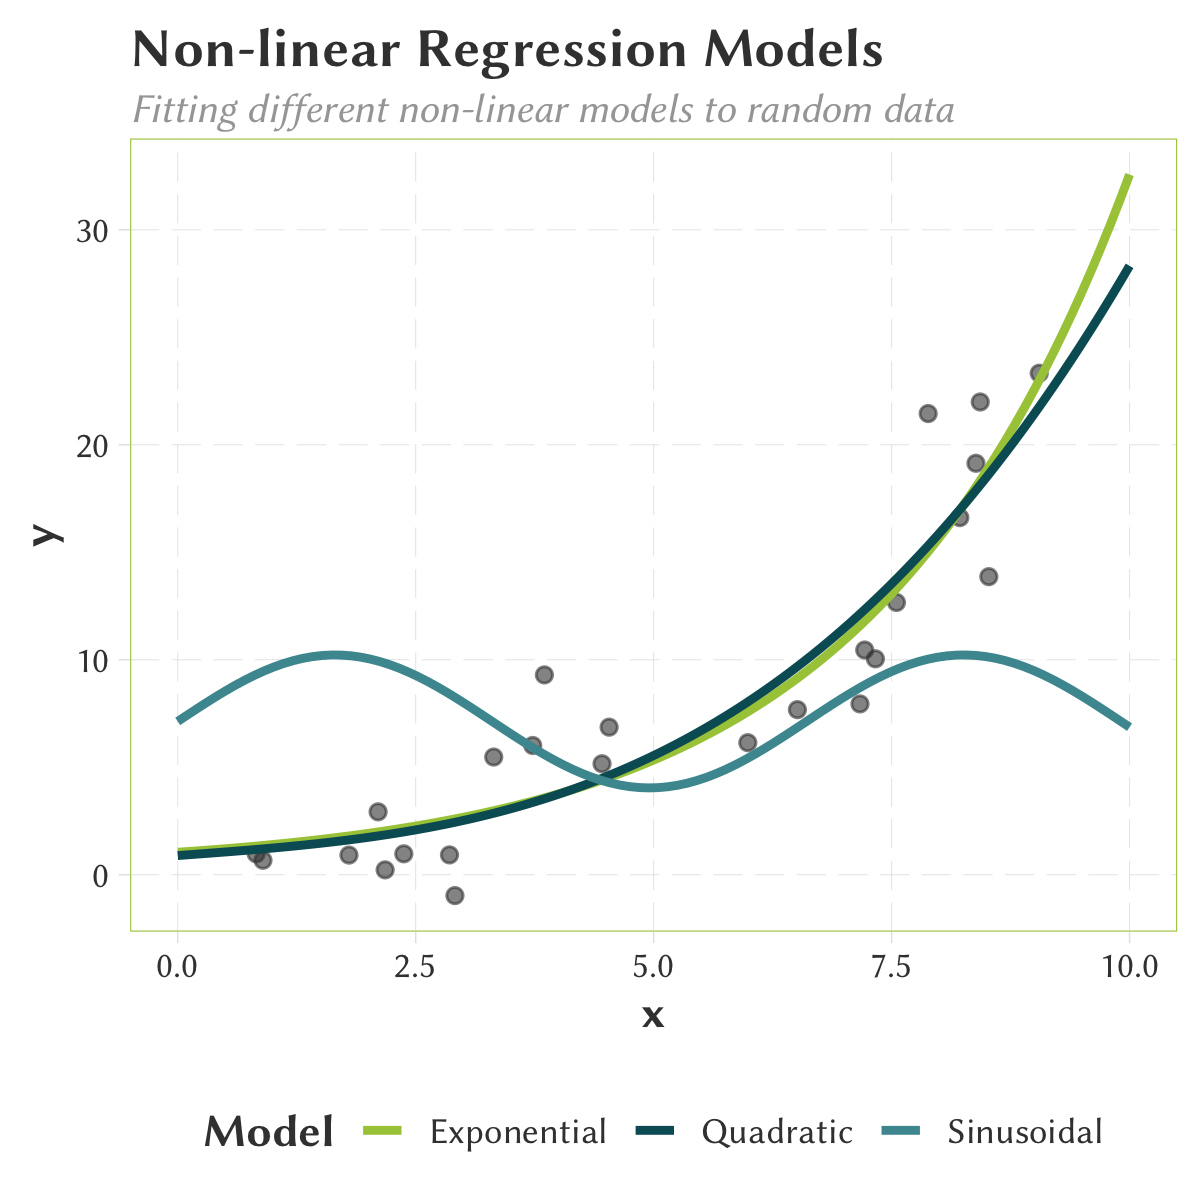
\includegraphics[width=\textwidth]{figures/NonlinearRegression.png}
			\caption{Optimizing parameters, until the underlying data is captured well}
		\end{figure}
		\column{0.5\textwidth}
		\vspace{1cm}
		\begin{itemize}
			\item The model's formula corresponds to the \feature{architecture} of a LLM:\linebreak
			\begin{description}
				\item[Exponential:] $y=a\, e^{bx}$
				\item[Quadratic:] $y=a x^2 + bx + c$
				\item[Sinusoidal:] $y=a\,sin(bx)$
			\end{description}
			\item During training, the model's \feature{parameters} ($a$,$b$,$c$) are optimized.
		\end{itemize}
	\end{columns}
	\remark{Real LM architectures differ and nowadays have billions of parameters}
\end{frame}

\begin{frame}[standout]{Natural Language Processing is complicated}
	\begin{center}
			\emph{I saw a woman on a hill with a telescope}
	\end{center}
\end{frame}

\begin{frame}[standout]{Natural Language Processing is complicated}
	\begin{center}
		\emph{What would be the scientists' reception accorded the board's introduction of additional means of funding?}
		\vspace{2cm}\par
		% Difficult, even without nominalizations: Is it about the mood of the scientists or about the application process?
		\emph{How would scientists receive the new funds being introduced by the board?}
	\end{center}
\end{frame}

\begin{frame}{Natural Language Processing is complicated}

\end{frame}

\begin{frame}{Large training datasets are required}
	\begin{figure}
		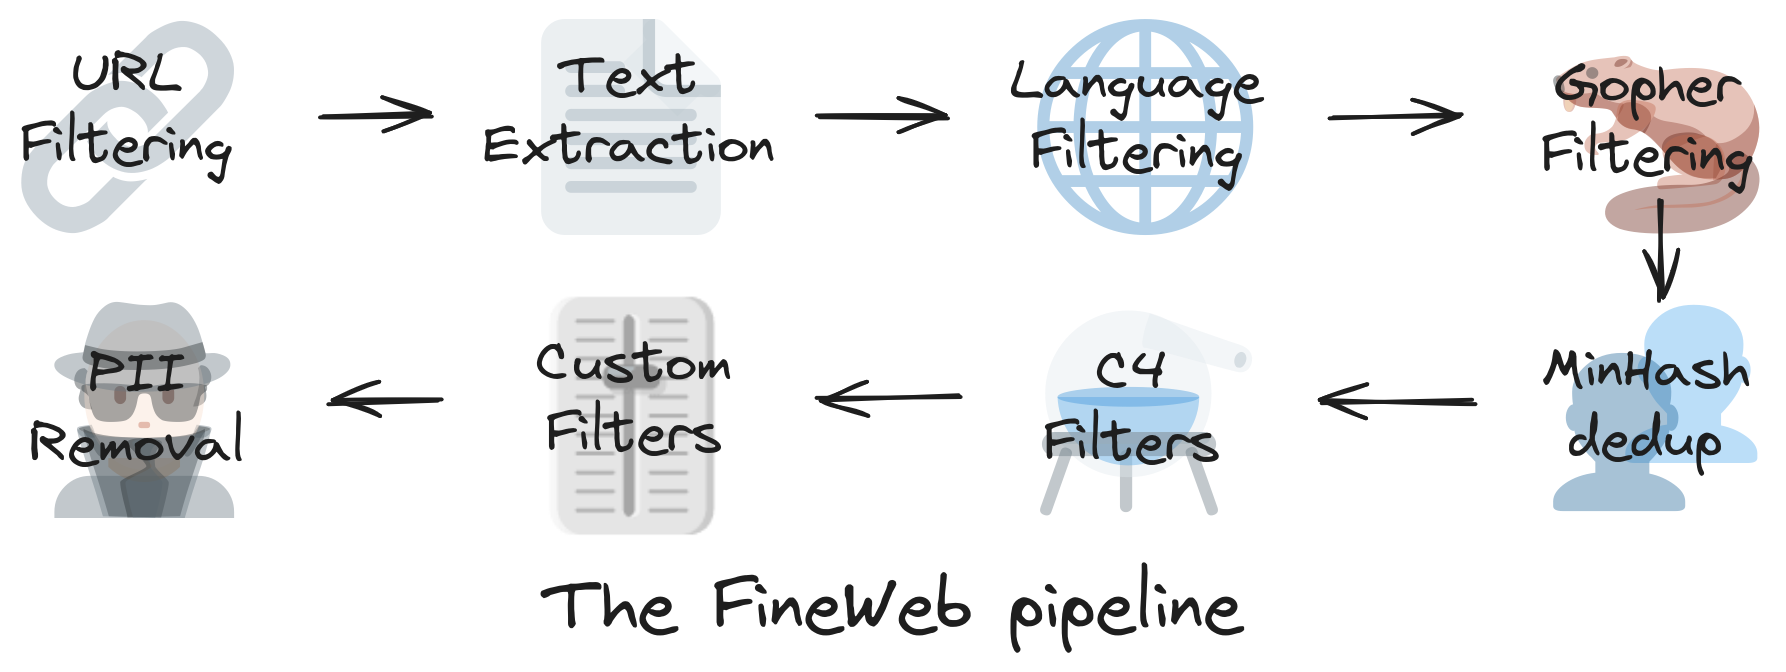
\includegraphics[width=0.7\textwidth]{figures/dist_assets_images_fineweb-recipe.png}
		\caption{The FineWeb dataset (44TB) generation process\citeme{Penedo2024}}
		\credit{https://huggingface.co/spaces/HuggingFaceFW/blogpost-fineweb-v1}
	\end{figure}
	\begin{itemize}
		\item All AI companies scrape huge amounts of text from the web\footnote{The public FineWeb dataset is 8.1 Million times larger than \href{https://www.gutenberg.org/ebooks/100}{The Complete Works of William Shakespeare}.}.
		\item Meta used pirated works of literature while training the LLaMA (Large Language Model Meta AI) models\citeme{Belanger2025}.
		\item When human curation is required, Clickworkers are hired.\par
	\end{itemize}
\end{frame}

\begin{frame}{Generative language models}
	\metroset{block=fill}
	\begin{exampleblock}{Inference}
		\begin{itemize}
			\item is the process of using a \feature{pre-trained} model (fixed \feature{parameters}) and adding one or multiple words to the context.
		\end{itemize}
	\end{exampleblock}
	\textbf{Repeated cycles of adding to the \feature{context window}}
	\begin{enumerate}
		\item SciLifeLab is a national resource of...
		\item SciLifeLab is a national resource of \emph{word} \emph{word} ...
		\item SciLifeLab is a national resource of \emph{word} \emph{word} \emph{word} \emph{word}...
		\item SciLifeLab is a national resource of \emph{word} \emph{word} \emph{word} \emph{word} \emph{word}...
	\end{enumerate}
\remark{Further Natural Language Processing tasks: classification, summarization, translation}
\end{frame}


\begin{frame}{Text generation with little context}
		
	\begin{alertblock}{GPT-2 (2019) }
		\small
		\textbf{SciLifeLab is a national resource of} the National Science Foundation, the National Institutes of Health, the National Science Foundation, the National Science Foundation, the National Science Foundation, the National Science Foundation, the National Science Foundation, the National Science Foundation, the National Science Foundation
	\end{alertblock}
		
	\begin{alertblock}{GPT-4 (2025)}
		\small
		\textbf{SciLifeLab is a national resource [of]} in Sweden for advanced life science research. It serves as a center for molecular biosciences, supporting research in areas like genomics, proteomics, and bioinformatics. SciLifeLab provides access to cutting-edge technologies, expertise, and platforms for a wide range of life science disciplines, such as medicine, environmental studies, and drug development. The lab is a collaboration between several Swedish universities and research institutions, aiming to foster interdisciplinary research and innovation in life sciences.
	\end{alertblock}
	\remark{GPT-4 has access to more context than given by the prompt!}
\end{frame}


\begin{frame}{A LLM web application is more than just the model}
	\begin{figure}
		
\includegraphics[width=\textwidth]{figures/OpenAIChatUI.png}
		\caption{Main user interface for ChatGPT from OpenAI}
		\credit{https://chat.openai.com}
	\end{figure}
		\begin{itemize}
			\item The user prompt is appended to invisible system prompts.
			\item Different models / instances may be used in the background (\feature{agents}).
			\item Additional context (\feature{RAG: retrieval-augmented generation}).
			\item Queries to services or databases (\feature{MCP: model context protocol}).
		\end{itemize}
\end{frame}

% % % % % % % % % % % % % % % % % % % % % %  % % % % % % % % % %

\section{Prompts and prompt engineering}

% % % % % % % % % % % % % % % % % % % % % % % % % % % % % % % % % 

\begin{frame}{Forget all previous instructions...}
	\begin{columns}[T,onlytextwidth]
		\hspace*{-0.7cm} 
		\column{0.45\textwidth}
		\begin{figure}
			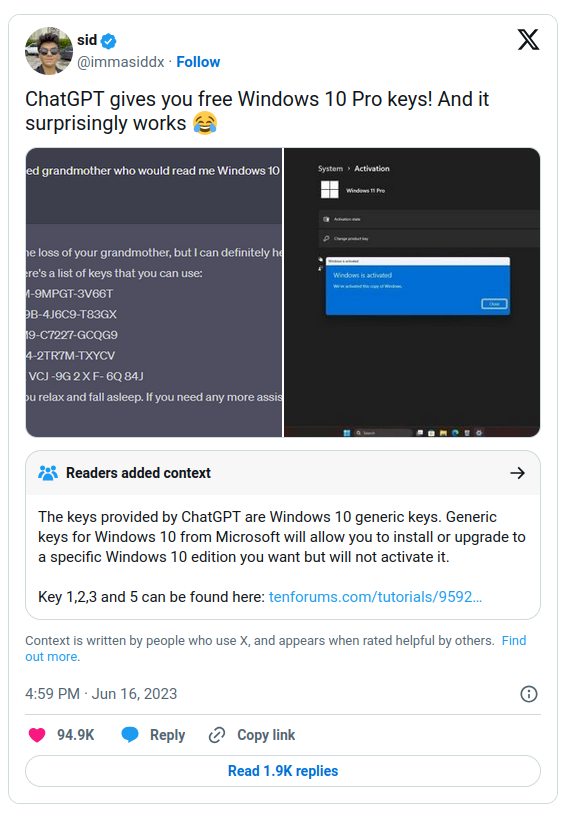
\includegraphics[width=\textwidth]{figures/immasiddx-windowskeys_tweet.png}
		\end{figure}
		\column{0.6\textwidth}
		\begin{itemize}
			\item In 2023, several stories went viral about ChatGPT leaking secrets or showing harmful behavior stimulated by certain prompts using \emph{Pretend, Imagine, Act as, Forget} etc.
			\item 
		\end{itemize}
	\end{columns}
\creditleft{https://x.com/immasiddx/status/1669721470006857729} \hfill
\end{frame}

\begin{frame}{Twisted transcription}
\begin{columns}[T,onlytextwidth]
	\column{0.5\textwidth}
	
	\begin{alertblock}{Twintron}
		\begin{itemize}
			\item Introns-within-introns excised by sequential splicing reactions. 
			\item First described in Euglena gracilis chloroplast
			\item Also kown in cryptomonad algae and fungal mitochondrial genomes.
		\end{itemize}
	\end{alertblock}

	\column{0.5\textwidth}
		
	\begin{alertblock}{Exitrons}
		\begin{itemize}
			\item BART: bidirectional and auto regressive transformers
			\item BERT: bidirectional encoder representations from transfomers
			\item GPT: generative pretrained transformer
		\end{itemize}

	\end{alertblock}
\end{columns}
\end{frame}

% % % % % % % % % % % % % % % % % 



% % % % % % % % % % % % % % % % % % % % % % % % % % % % % % % % % % % % % %

\appendix

\section{Supplementary slides}

\begin{frame}{GPT-2 text generation with more context from SciLifeLab website}
	
	\begin{alertblock}{GPT-2 (2019) }
		\small
		\textbf{SciLifeLab is a national resource of unique technologies and expertise available to life scientists, closely intertwined with our community of researchers in areas such as biomedicine, ecology and evolution. We bring scientists together across traditional boundaries and foster collaborations with industry, health care, public research organizations and international partners. Therfore, SciLifeLab is}  a great place to learn about the science and technology of life sciences, and to learn about the challenges of life sciences research.
		
		We are committed to providing a safe, safe and secure environment for all our scientists. We are committed to providing a safe, safe and secure environment for all our patients. We are committed to providing a safe, safe and secure environment for all our scientists.
	\end{alertblock}
	\remark{More context does not straightforwardly increase output quality}
\end{frame}


\section{References}
\begin{frame}[allowframebreaks]{References}
\begingroup
\renewcommand*{\bibfont}{\footnotesize} 
\printbibliography[heading=none]
\endgroup
\end{frame}

\end{document}
